% Generation cost tables.
% Source: tracking/pricing.py (DEFAULT_PRICING), the benchmark's own pricing
% table used to compute each run's cost_usd.
%
% Required packages:
%   \usepackage{booktabs}
%   \usepackage{graphicx}
%
% Figures are regenerated with: python "Code/Testing/plot_generation_costs.py"
% (writes to Artifacts/Figures/). \includegraphics paths below assume Figures/
% sits next to the compiled main.tex, per the document's actual layout.

% ---------------------------------------------------------------------------
% Recorded billing rates, the 11 models in the benchmark roster
% ---------------------------------------------------------------------------
\begin{table}[htbp]
  \centering
  \caption{Billing rates by model (USD per 1M tokens, standard tier)}
  \label{tab:cost-rates}
  \begin{tabular}{llrr}
    \toprule
    Provider & Model & Input & Output \\
    \midrule
    Anthropic & Claude Haiku 4.5   & \$1.00 & \$5.00  \\
    Anthropic & Claude Sonnet 5    & \$3.00 & \$15.00 \\
    Anthropic & Claude Opus 4.8    & \$5.00 & \$25.00 \\
    \cmidrule(lr){1-4}
    Google & Gemini 2.5 Flash-Lite & \$0.10 & \$0.40  \\
    Google & Gemini 3.1 Flash-Lite & \$0.25 & \$1.50  \\
    Google & Gemini 3.5 Flash      & \$1.50 & \$9.00  \\
    Google & Gemini 3.1 Pro Preview & \$2.00 & \$12.00 \\
    \cmidrule(lr){1-4}
    OpenAI & GPT-5.4 Nano  & \$0.20 & \$1.25  \\
    OpenAI & GPT-5.4 Mini  & \$0.75 & \$4.50  \\
    OpenAI & GPT-5.4       & \$2.50 & \$15.00 \\
    OpenAI & GPT-5.5       & \$5.00 & \$30.00 \\
    \bottomrule
  \end{tabular}
  \par\smallskip
  \footnotesize Rates as recorded in \texttt{tracking/pricing.py}'s \texttt{DEFAULT\_PRICING} (verified against each provider's official pricing page, 2026-07), the same table the benchmark uses to compute each run's \texttt{cost\_usd}. Standard/base tier only -- no prompt-caching, batch, or long-context-tier discounts applied. Anthropic's Sonnet 5 has an introductory \$2/\$10 rate through 2026-08-31; the standard \$3/\$15 rate is stored and used here. Providers ordered alphabetically; within a provider, ordered by size tier (small, medium, large) to match the size-tier grouping used in the failure tables.
\end{table}

% ---------------------------------------------------------------------------
% Mean token consumption and generation cost per run, by model (L3/L4 base)
% Source figure: Artifacts/Figures/cost_tokens_by_model.pdf
% ---------------------------------------------------------------------------
\begin{figure}[htbp]
  \centering
  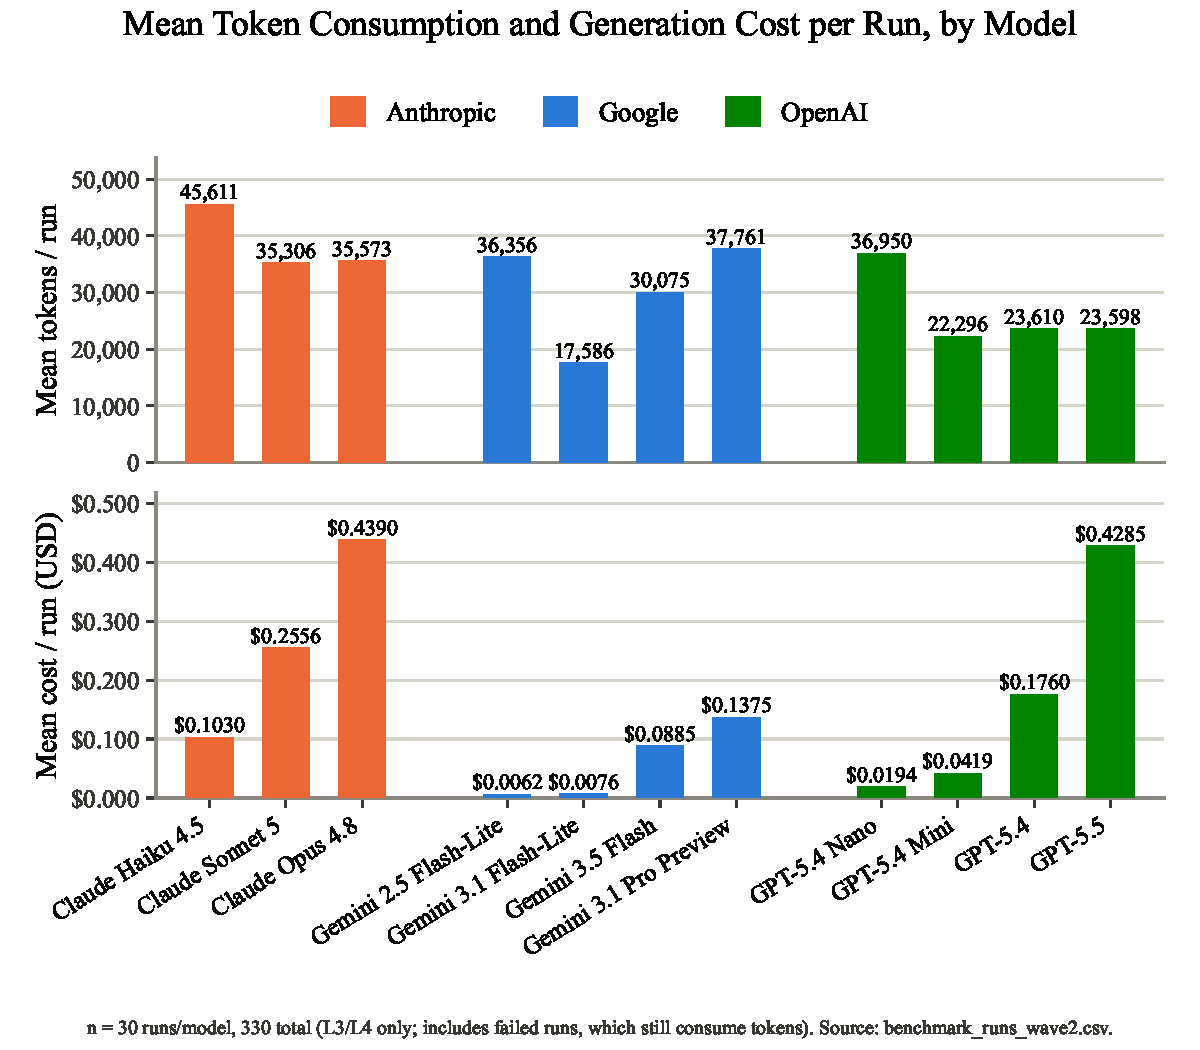
\includegraphics[width=\textwidth]{Figures/cost_tokens_by_model.pdf}
  \caption{Mean token consumption and generation cost per run, by model (n=30 runs/model, 330 total; L3/L4 only, per-model averages include failed runs, which still consume tokens). Bars colored by provider: orange = Anthropic, blue = Google, green = OpenAI.}
  \label{fig:cost-tokens-by-model}
\end{figure}

% ---------------------------------------------------------------------------
% Same figure, L1 (outline) runs only -- L1 never failed in this dataset;
% compare against the figure above to weigh whether L1 belongs folded into
% an overall cost figure or is better reported separately.
% Source figure: Artifacts/Figures/cost_tokens_by_model_L1.pdf
% ---------------------------------------------------------------------------
\begin{figure}[htbp]
  \centering
  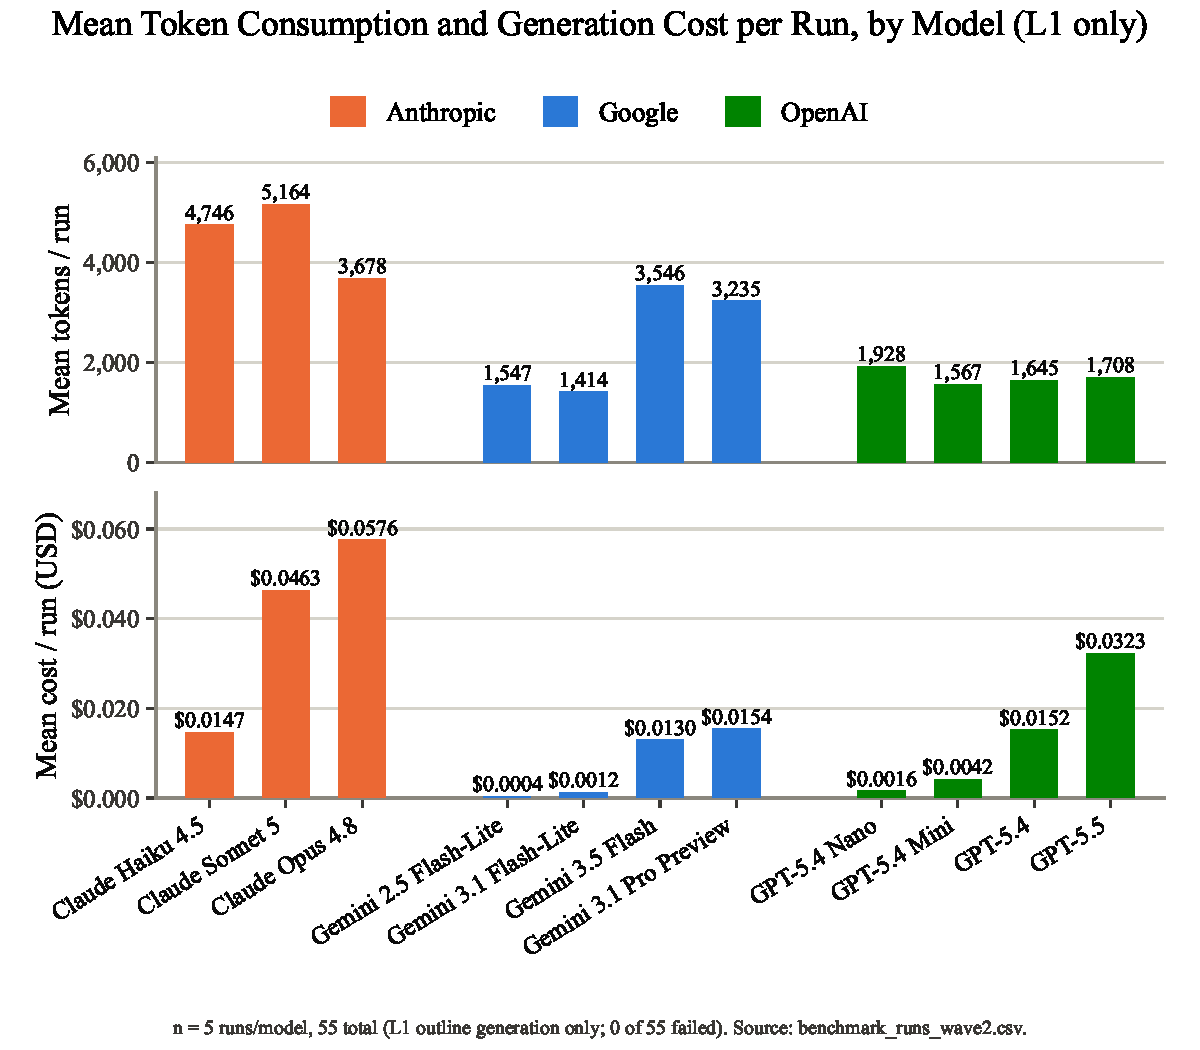
\includegraphics[width=\textwidth]{Figures/cost_tokens_by_model_L1.pdf}
  \caption{Mean token consumption and generation cost per run, by model, L1 (outline) runs only (n=5 runs/model, 55 total; 0 of 55 failed). Same axes and provider coloring as Figure~\ref{fig:cost-tokens-by-model}, roughly an order of magnitude lower on both.}
  \label{fig:cost-tokens-by-model-l1}
\end{figure}
